\section{Experiments}\label{experiment}
We employ \computerrl on \glm~\citep{glm2024chatglm} and \glmv~\citep{hong2025glm}, to produce \model-9b.
We conduct extensive experiments across various scenarios to evaluate \model's performance within the computer environment.

\input{tables/osworld}

\subsection{Main Results}\label{exp:osworld}
To closely reflect the real user experience, we evaluate \model on the OSWorld~\citep{xie2024osworld} and \href{https://xlang.ai/blog/osworld-verified}{OSWorld-Verified} benchmark, comparing its performance against state-of-the-art models, including CUA~\citep{cua2025}, Claude-4~\citep{claude2}, and UI-TARS~\citep{qin2025ui}, among others. The comparative results are in Table~\ref{tab:osworld}.
The results indicate that \model achieves superior performance across a range of domains, with its advantages most pronounced in the challenging multi-apps setting. Moreover, by employing the API-GUI strategy, \model can accomplish tasks using at most \textbf{1/3} of the steps required by the strongest baseline approaches, demonstrating remarkable gains in execution efficiency. These results underscore the potential of \computerrl to advance the state of the art in computer automation across various applications.

\subsection{Office Application Performance}
As a critical interface for delivering and presenting, office application constitutes an important testbed for evaluating computer use agents. 
To assess agent performance in this domain, we curate a set of 180 challenging tasks from three sources: SpreadsheetBench~\citep{ma2024spreadsheetbench}, PPTC~\citep{guo2023pptc}, and in-house developed Writer domain tasks. These tasks are adapted as necessary to integrate them into the OSWorld framework. The resulting benchmark, termed \textbf{OfficeWorld}, enables systematic measurement of agent capabilities in office-oriented scenarios. The results are in Table~\ref{tab:officeworld}.

\begin{table*}[h!]
\centering
\caption{\model performance on OfficeWorld compared to common baselines. We employ the same framework (with tools) and test settings to ensure a fair comparison.}
\vspace{-3mm}
\renewcommand\tabcolsep{12pt}
% \renewcommand\arraystretch{0.9}
\label{tab:officeworld}
\resizebox{\columnwidth}{!}{
\begin{tabular}{@{}p{7.5cm}cccc@{}}
\specialrule{1.0pt}{1.0pt}{1.0pt}
\textbf{Agent Model} & \textbf{Word} & \textbf{Excel} & \textbf{PPT} & \textbf{Average} \\
\specialrule{1.0pt}{1.0pt}{1.0pt}
DeepSeek-V3.1~\citep{liu2024deepseek} & 6.7 & 35.0 & 21.7 & 21.1 \\
DeepSeek-R1~\cite{guo2025deepseek} & 13.3 & 36.7 & 18.3 & 22.8 \\
Claude 3.7 Sonnet~\citep{claude2} & 15.0 & 25.0 & 25.0 & 21.7 \\
Claude 4.0 Sonnet~\citep{claude2} & 18.3 & 35.0 & 20.0 & 24.4 \\
Gemini-2.5-Pro~\citep{team2023gemini} & 5.0 & 11.7 & 20.0 & 12.2 \\
GPT-4o~\citep{hurst2024gpt} & 18.3 & 21.7 & 8.3 & 16.1 \\
GPT-4.1~\citep{achiam2023gpt} & 21.7 & 25.0 & 28.3 & 25.0 \\
OpenAI o3~\citep{jaech2024openai} & \underline{23.3} & 36.7 & \underline{41.7} & 33.9 \\
\midrule[\heavyrulewidth]
\multicolumn{4}{@{}l}{\computerrl \textit{(ours)}} \\
\quad w/ \glm & 21.7 & \textbf{58.3} & \textbf{43.3} & \underline{41.1} \\
\quad w/ \glmv & \textbf{30.0} & \textbf{58.3} & \underline{41.7} & \textbf{43.3} \\
\specialrule{1.0pt}{1.0pt}{1.0pt}
\end{tabular}
}
\end{table*}

\subsection{Ablation Study}
To evaluate the influence of various algorithms and training datasets on agent performance, we present an ablation study on the OSWorld benchmark in Table~\ref{tab:ablation_study}. 

\begin{table}[t]
\caption{Ablation study on framework designs and training methods. We categorize OSWorld into five distinct domains to facilitate a more granular comparison of the effects of different strategies across various domains.}
\vspace{-2mm}
\label{tab:ablation_study}
\centering
\renewcommand\tabcolsep{12pt}
\resizebox{\columnwidth}{!}{
\begin{tabular}{@{}lcccccc@{}}
\toprule
Method & OS & Office & Daily & Professional & Workflow & Avg. \\ 
\midrule
\multicolumn{7}{c}{Framework Ablation (w/ \gptfouro)}\\  
\midrule
GUI Only & 41.7 & 6.2 & 12.3 & 14.3 & 7.5 & 11.2 \\
API-GUI & 52.6 & 27.9 & 25.7 & 41.6 & 10.8 & 26.2 \\
\midrule
\multicolumn{7}{c}{Training Ablation}\\ 
\midrule
Untrained & 20.8 & 17.2 & 19.7 & 22.9 & 3.3 & 15.2 \\
+) Behavior Cloning & 54.2 & 35.0 & 37.2 & 45.8 & 10.8 & 31.9 \\
+) RL Phase 1 & 83.3 & 46.1 & 45.1 & 56.3 & 16.1 & 42.0 \\
+) \rlmethod & 75.0 & 42.3 & 50.6 & 52.1 & 18.9 & 41.5 \\
+) RL Phase 2 & \textbf{83.3} & \textbf{46.2} & \textbf{46.7} & \textbf{60.4} & \textbf{27.2} & \textbf{45.8} \\
\bottomrule
\end{tabular}
}
\end{table}

\vpara{Framework Ablation.}
We compare the performance of the GUI-only approach with our proposed API-GUI paradigm using \gptfouro. The results demonstrate that the API-GUI paradigm substantially outperforms the GUI-only baseline across all domains. Specifically, the API-GUI strategy achieves an average success rate of 26.2\%, representing a 134\% improvement over the GUI-only approach (11.2\%). The most significant gains are observed in the Office (27.9\% vs. 6.2\%) and Professional (41.6\% vs. 14.3\%) domains, where API-GUI provides 350\% and 191\% improvements, respectively. These results validate our core hypothesis that combining API calls with GUI interactions enables more efficient and reliable task execution, particularly for complex professional workflows that benefit from programmatic control.

\begin{figure}[t]
    \centering
    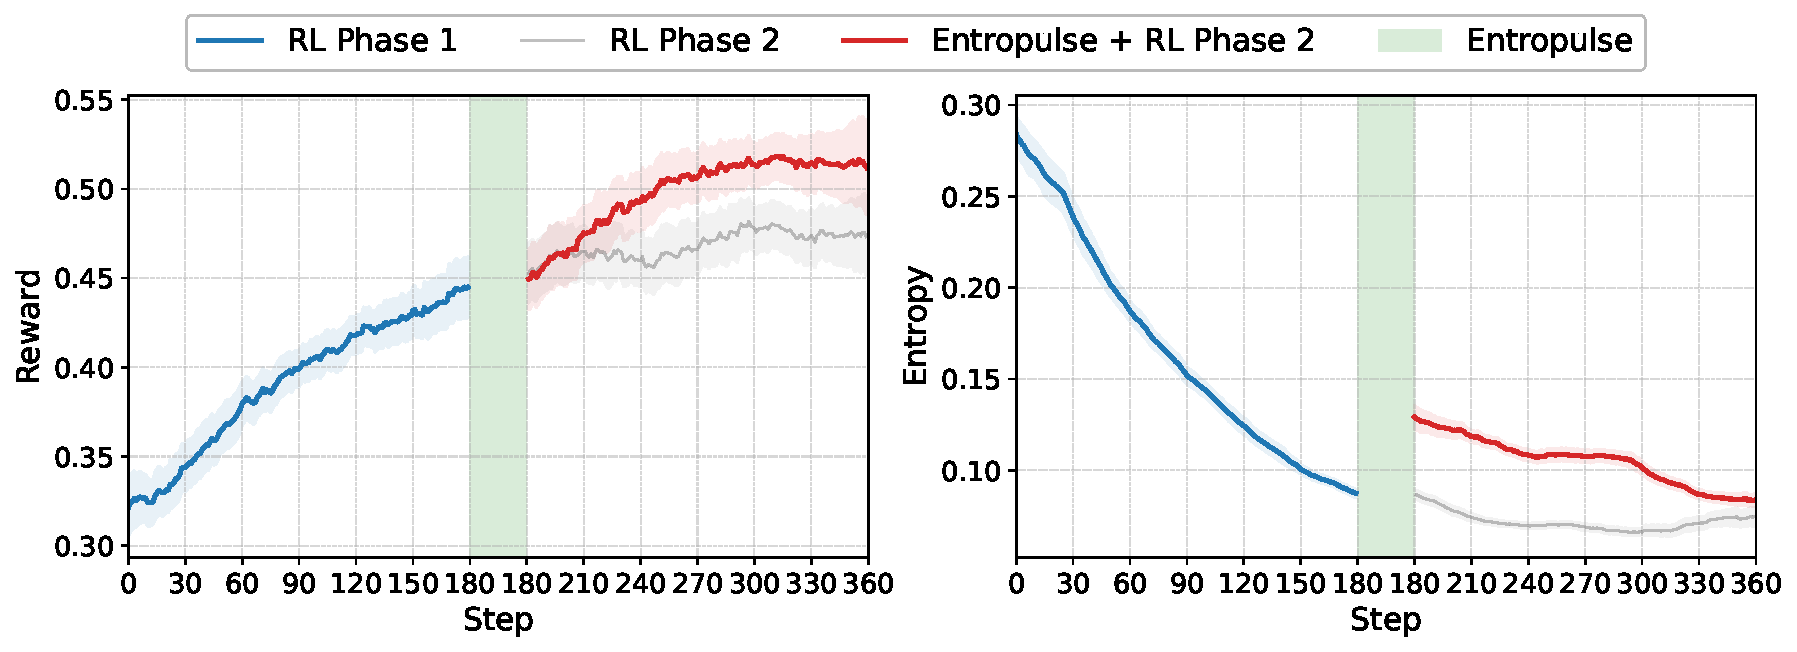
\includegraphics[width=\linewidth]{images/rl_curve_reward_entropy_exp.pdf}
    \vspace{-7mm}
    \caption{\computerrl training curves of reward (left) and entropy (right) with 95\% confidence intervals. The red line denotes the training with entropy recovery via \rlmethod after the first RL stage, while the grey line denotes continued training with only reference resetting.}
    \label{figs:trending}
\end{figure}

\vpara{Training Ablation.}
We study the progressive impact of different training stages using \qwen. 
Starting from the backbone, Behavior Cloning (BC) establishes a solid foundation with 31.9\%. The first RL phase (RL1) yields substantial gains, increasing the performance to 42.0\% (+10.1\%). 
Interestingly, \rlmethod phase maintains similar performance (41.5\%) while significantly increasing action entropy, which enhances exploration diversity and enables the final RL2 phase to achieve further improvements. 
The RL2 phase achieves the best performance at 45.8\% (+3.8\% from RL1), benefiting from the increased exploration capacity introduced by \rlmethod. 
Notably, the Workflow domain shows the most dramatic improvement throughout training (10.8\% → 27.2\%), while the other domains maintain consistently high performance, highlighting the importance of multi-stage training.



\vpara{RL Scalability.}
We present the RL training reward and entropy curves in Figure~\ref{figs:trending} to study the impact of \rlmethod on the extended RL training dynamics.
After the first RL phase converges, we compare the second RL phase with and without \rlmethod. To ensure a fair comparison, we reset the reference model in both scenarios. 

The results demonstrate that incorporating \rlmethod increases the model’s entropy, thereby restoring its exploratory capacity. This enhanced exploration substantially scales the effective training steps, ultimately leading to improved overall performance.

\subsection{Case Study and Error Analysis}

\begin{wrapfigure}[13]{r}{0.28\textwidth}
    \vspace{-13mm}
    \centering
    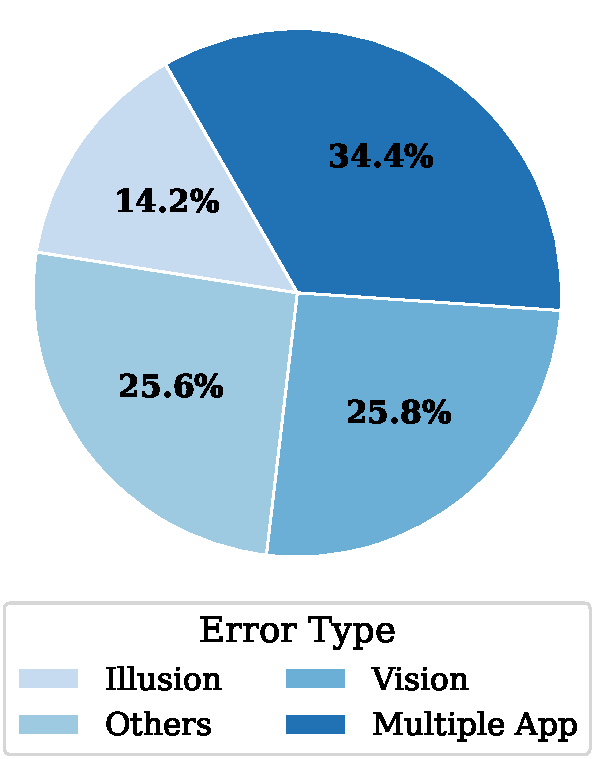
\includegraphics[width=0.9\linewidth]{images/error_analysis.pdf}
    \caption{Error distribution.}
    \label{figs:error_analysis}
\end{wrapfigure}

We conduct a case study in the desktop environment to identify potential avenues for system optimization. Although our model exhibits robust performance across most scenarios, several limitations have been identified. In particular, errors encountered during task execution can be categorized into four primary types: visual perception errors, multi-application coordination failures, operational illusions, and other errors. The distribution of these error types is presented in Figure~\ref{figs:error_analysis}. 

Additional representative examples, including both successful and unsuccessful cases, are provided in Appendix~\ref{apdx:demo} to further illustrate the model's capabilities and limitations.
